\documentclass[12pt]{report}
\usepackage[utf8]{inputenc}
\usepackage[russian]{babel}
%\usepackage[14pt]{extsizes}
\usepackage{listings}
\usepackage{amsmath}
\usepackage[justification=centering]{caption}

\lstdefinelanguage{Nim}{
  comment=[l]{//},
  commentstyle={\color{gray}\ttfamily},
  emph={delegate, filter, first, firstOrNull, forEach, lazy, map, mapNotNull, println, return@},
  emphstyle={\color{OrangeRed}},
  identifierstyle=\color{black},
  keywords={abstract, actual, as, as?, break, by, class, companion, continue, data, do, dynamic, else, enum, expect, false, final, for, proc, get, if, import, in, interface, internal, is, null, object, override, package, private, public, return, set, super, suspend, this, throw, true, try, typealias, val, var, vararg, when, where, while},
  keywordstyle={\color{blue}\bfseries},
  morecomment=[s]{/*}{*/},
  morestring=[b]",
  morestring=[s]{"""*}{*"""},
  ndkeywords={@Deprecated, @JvmField, @JvmName, @JvmOverloads, @JvmStatic, @JvmSynthetic, seq, Byte, Double, Float, int, Integer, Iterable, Long, Runnable, Short, String},
  ndkeywordstyle={\color{orange}\bfseries},
  sensitive=true,
  stringstyle={\color{green}\ttfamily},
}

% Для листинга кода:
\lstset{ %
language=Nim,                 % выбор языка для подсветки (здесь это С)
basicstyle=\footnotesize\sffamily, % размер и начертание шрифта для подсветки кода
numbers=left,               % где поставить нумерацию строк (слева\справа)
numberstyle=\tiny,           % размер шрифта для номеров строк
stepnumber=1,                   % размер шага между двумя номерами строк
numbersep=5pt,                % как далеко отстоят номера строк от подсвечиваемого кода
showspaces=false,            % показывать или нет пробелы специальными отступами
showstringspaces=false,      % показывать или нет пробелы в строках
showtabs=false,             % показывать или нет табуляцию в строках
frame=single,              % рисовать рамку вокруг кода
tabsize=2,                 % размер табуляции по умолчанию равен 2 пробелам
captionpos=t,              % позиция заголовка вверху [t] или внизу [b] 
breaklines=true,           % автоматически переносить строки (да\нет)
breakatwhitespace=false, % переносить строки только если есть пробел
escapeinside={\#*}{*)}   % если нужно добавить комментарии в коде
}

\usepackage{hyperref}
\hypersetup{
    linktoc=all,     %set to all if you want both sections and subsections linked
    linkcolor=blue,  %choose some color if you want links to stand out
}

% Для измененных титулов глав:
\usepackage{titlesec, blindtext, color} % подключаем нужные пакеты
\definecolor{gray75}{gray}{0.75} % определяем цвет
\newcommand{\hsp}{\hspace{20pt}} % длина линии в 20pt
% titleformat определяет стиль
\titleformat{\chapter}[hang]{\Huge\bfseries}{\thechapter\hsp\textcolor{gray75}{|}\hsp}{0pt}{\Huge\bfseries}

% plot
\usepackage{pgfplots}
\usepackage{filecontents}
\usetikzlibrary{datavisualization}
\usetikzlibrary{datavisualization.formats.functions}

\begin{filecontents}{KB11.dat}
100 4692982
200 49620266
300 178730542
400 429056319
500 856058247
\end{filecontents}

\begin{filecontents}{KB21.dat}
100 6144734
200 56025172
300 199925329
400 456832433
500 737473554
\end{filecontents}

\begin{filecontents}{KB31.dat}
100 6125329
200 58077386
300 206518482
400 561695647
500 673711435
\end{filecontents}

\begin{filecontents}{KB12.dat}
100 4250527
200 50728798
300 186202130
400 436860056
500 870833440
\end{filecontents}

\begin{filecontents}{KB22.dat}
100 4315274
200 34809356
300 120880876
400 248104438
500 576761740
\end{filecontents}

\begin{filecontents}{KB32.dat}
100 2910312
200 18273241
300 61885504
400 137340969
500 267199177
\end{filecontents}

\begin{filecontents}{KB14.dat}
100 4485824
200 51678241
300 176448578
400 436787067
500 850999256
\end{filecontents}

\begin{filecontents}{KB24.dat}
100 4239416
200 28600648
300 80224609
400 208705553
500 485612161
\end{filecontents}

\begin{filecontents}{KB34.dat}
100 2969518
200 10260636
300 31277241
400 70302333
500 151094601
\end{filecontents}

\begin{filecontents}{KB18.dat}
100 4403638
200 52234883
300 177331754
400 442171563
500 877219464
\end{filecontents}

\begin{filecontents}{KB28.dat}
100 5304634
200 26568390
300 107137650
400 337629280
500 883596315
\end{filecontents}

\begin{filecontents}{KB38.dat}
100 3712704
200 11046163
300 31637714
400 58383234
500 117636357
\end{filecontents}

\begin{filecontents}{KB116.dat}
100 4463337
200 50528949
300 175677695
400 433177913
500 831773652
\end{filecontents}

\begin{filecontents}{KB216.dat}
100 7381390
200 32361454
300 110593792
400 342768739
500 887656714
\end{filecontents}

\begin{filecontents}{KB316.dat}
100 4981564
200 17479130
300 44960321
400 68839512
500 100236284
\end{filecontents}





\begin{document}
\begin{titlepage}
	\fontsize{12pt}{12pt}\selectfont
	\noindent \begin{minipage}{0.15\textwidth}
		
\includegraphics[width=\linewidth]{inc/img/b_logo.jpg}
	\end{minipage}
	\noindent\begin{minipage}{0.9\textwidth}\centering
		\textbf{Министерство науки и высшего образования Российской Федерации}\\
		\textbf{Федеральное государственное бюджетное образовательное учреждение высшего образования}\\
		\textbf{«Московский государственный технический университет имени Н.Э.~Баумана}\\
		\textbf{(национальный исследовательский университет)»}\\
		\textbf{(МГТУ им. Н.Э.~Баумана)}
	\end{minipage}
	
	\noindent\rule{15cm}{3pt}
	\newline\newline
	\noindent ФАКУЛЬТЕТ \underline{~~~~~~~~~~~~~~~~«Информатика и системы управления»~~~~~~~~~~~~~~~~} \newline\newline
	\noindent КАФЕДРА \underline{«Программное обеспечение ЭВМ и информационные технологии»}\newline\newline\newline\newline\newline\newline\newline
	
	
	\begin{center}
		\Large\textbf{Отчет по лабораторной работе №4 по курсу "Анализ алгоритмов"}\newline
	\end{center}
	
	\noindent\textbf{Тема} \underline{Реализация параллельного алгоритма Копперсмита-Винограда}\newline\newline\newline
	\noindent\textbf{Студент} \underline{Якуба Д. В.}\newline\newline
	\noindent\textbf{Группа} \underline{ИУ7-53Б}\newline\newline
	\noindent\textbf{Оценка (баллы)} \underline{~~~~~~~~~~~~~~~~~~~}\newline\newline
	\noindent\textbf{Преподаватели} \underline{Волкова Л.Л., Строганов Ю.В.}\newline
	
	\begin{center}
		\vfill
		Москва~---~\the\year
		~г.
	\end{center}
\end{titlepage}

\setcounter{page}{2}

\tableofcontents

\newpage
\chapter*{Введение}
\addcontentsline{toc}{chapter}{Введение}
\section*{Цель лабораторной работы}
Изучение параллельных вычислений.
\section*{Задачи лабораторной работы}
\begin{enumerate}
\item изучение последовательного и двух параллельных реализаций алгоритмов Копперсмита-Винограда;
\item реализация последовательного и двух параллельных алгоритмов Копперсмита-Винограда;
\item проведение сравнительного анализа временных характеристик реализованных алгоритмов на основе экспериментальных данных;
\item подготовка отчёта по лабораторной работе;
\item получение практических навыков реализации алгоритмов на ЯП Nim.
\end{enumerate}
\section*{Определение}
Многопоточность — это способность центрального процессора (CPU) или одного ядра в многоядерном процессоре одновременно выполнять несколько процессов или потоков, соответствующим образом поддерживаемых операционной системой.
Этот подход отличается от многопроцессорности, так как многопоточность процессов и потоков совместно использует ресурсы одного или нескольких ядер: вычислительных блоков, кэш-памяти ЦПУ или буфера перевода с преобразованием (TLB).

В тех случаях, когда многопроцессорные системы включают в себя несколько полных блоков обработки, многопоточность направлена на максимизацию использования ресурсов одного ядра, используя параллелизм на уровне потоков, а также на уровне инструкций.
Поскольку эти два метода являются взаимодополняющими, их иногда объединяют в системах с несколькими многопоточными ЦП и в ЦП с несколькими многопоточными ядрами.

Многопоточная парадигма стала более популярной с конца 1990-х годов, поскольку усилия по дальнейшему использованию параллелизма на уровне инструкций застопорились.
Смысл многопоточности — квазимногозадачность на уровне одного исполняемого процесса.
Значит, все потоки процесса помимо общего адресного пространства имеют и общие дескрипторы файлов. Выполняющийся процесс имеет как минимум один (главный) поток.

\chapter{Аналитическая часть}
Для проведения данной работы потребуется информация об алгоритме Копперсмита-Винограда умножения матриц.
\section{Алгоритм Копперсмита-Винограда умножения матриц}
Пусть даны две прямоугольные матрицы
\begin{equation}
	A_{lm} = \begin{pmatrix}
		a_{11} & a_{12} & \ldots & a_{1m}\\
		a_{21} & a_{22} & \ldots & a_{2m}\\
		\vdots & \vdots & \ddots & \vdots\\
		a_{l1} & a_{l2} & \ldots & a_{lm}
	\end{pmatrix},
	\quad
	B_{mn} = \begin{pmatrix}
		b_{11} & b_{12} & \ldots & b_{1n}\\
		b_{21} & b_{22} & \ldots & b_{2n}\\
		\vdots & \vdots & \ddots & \vdots\\
		b_{m1} & b_{m2} & \ldots & b_{mn}
	\end{pmatrix},
\end{equation}

тогда матрица $C$
\begin{equation}
	C_{ln} = \begin{pmatrix}
		c_{11} & c_{12} & \ldots & c_{1n}\\
		c_{21} & c_{22} & \ldots & c_{2n}\\
		\vdots & \vdots & \ddots & \vdots\\
		c_{l1} & c_{l2} & \ldots & c_{ln}
	\end{pmatrix},
\end{equation}

где
\begin{equation}
	\label{anal:eq}
	c_{ij} =
	\sum_{r=1}^{m} a_{ir}b_{rj} \quad (i=\overline{1,l}; j=\overline{1,n})
\end{equation}

будет называться произведением матриц $A$ и $B$.

Если посмотреть на результат умножения двух матриц, то видно, что каждый элемент в нем представляет собой скалярное произведение соответствующих строки и столбца исходных матриц.
Можно заметить также, что такое умножение допускает предварительную обработку, позволяющую часть работы выполнить заранее.

Рассмотрим два вектора $V = (v_1, v_2, v_3, v_4)$ и $W = (w_1, w_2, w_3, w_4)$.
Их скалярное произведение равно: $V \cdot W = v_1w_1 + v_2w_2 + v_3w_3 + v_4w_4$, что эквивалентно (\ref{for:new}):
\begin{equation}
    \label{for:new}
    V \cdot W = (v_1 + w_2)(v_2 + w_1) + (v_3 + w_4)(v_4 + w_3) - v_1v_2 - v_3v_4 - w_1w_2 - w_3w_4.
\end{equation}

Несмотря на то, что второе выражение требует вычисления большего количества операций, чем стандартный алгоритм: вместо четырех умножений - шесть, а вместо трех сложений - десять, выражение в правой части последнего равенства допускает предварительную обработку: его части можно вычислить заранее и запомнить для каждой строки первой матрицы и для каждого столбца второй, что позволит для каждого элемента выполнять лишь два умножения и пять сложений, складывая затем только лишь с 2 предварительно посчитанными суммами соседних элементов текущих строк и столбцов \cite{CoppersmithAndWinograd}.
Из-за того, что операция сложения быстрее операции умножения в ЭВМ, на практике алгоритм должен работать быстрее стандартного \cite{PogorelovVolkova}.

Важно заметить, что каждый элемент матрицы $C$ вычисляется независимо от других, а матрицы $A$ и $B$ не изменяются, поэтому для распараллеливания алгоритма будет достаточно распределить элементы каждой строки матрицы $C$ между потоками.

\section*{Вывод}
Был рассмотрен алгоритм умножения матриц Копперсмита-Винограда. В данной работе стоит задача реализации данного алгоритма в последовательном и параллельных видах. Независимость вычислений элементов результата даёт возможность реализовать несколько параллельных вариантов исполнения данного алгоритма.

\chapter{Конструкторская часть}
В данном разделе предоставлены схема алгоритма Копперсмита-Винограда и его схемы распараллеливания.
\section{Схема алгоритма Копперсмита-Винограда}
Схема алгоритма Копперсмита-Винограда предоставлена на рисунках \ref{img:winodradScheme}-\ref{img:colsPreComp}.

\begin{figure}
\begin{center}
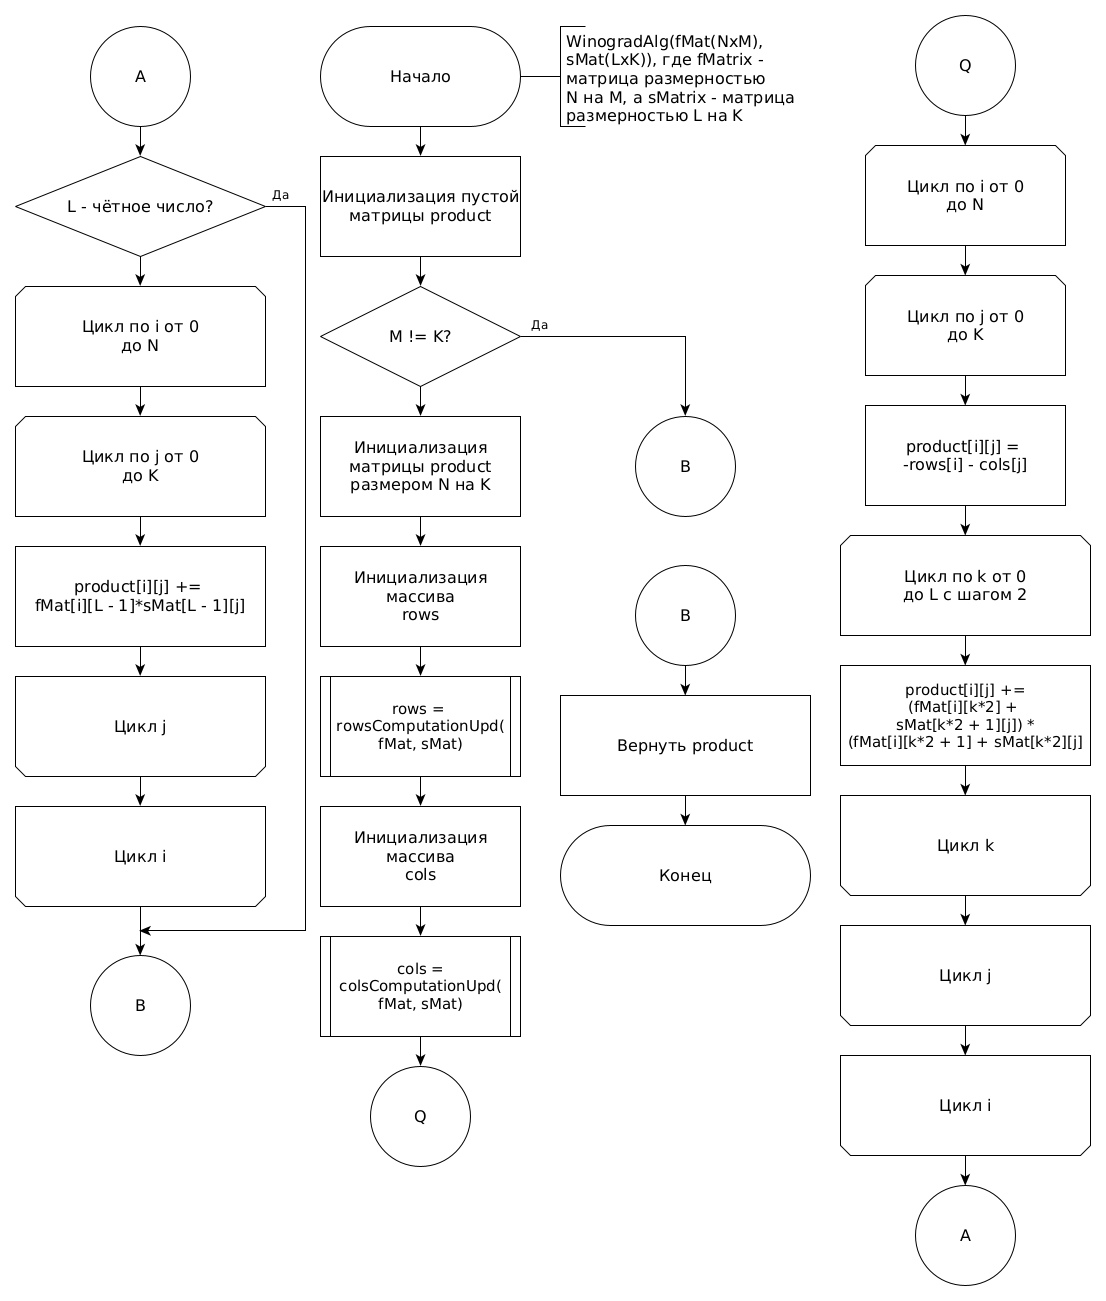
\includegraphics[scale=0.4]{inc/img/winogradScheme.png}
\captionsetup{justification=centering}
	\caption{Схема алгоритма Копперсмита-Винограда.}
	\label{img:winodradScheme}	
\end{center}
\end{figure}

\begin{figure}
\begin{center}
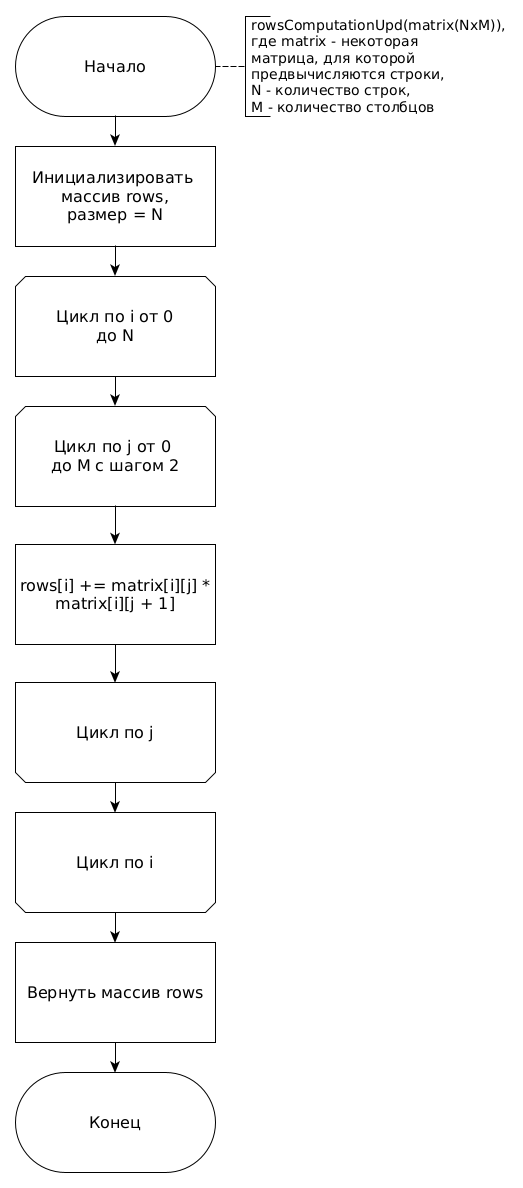
\includegraphics[scale=0.4]{inc/img/rowsCompUpd.png}
\captionsetup{justification=centering}
	\caption{Схема предрасчёта строк для алгоритма Копперсмита-Винограда.}
	\label{img:rowsPreComp}	
\end{center}
\end{figure}

\begin{figure}
\begin{center}
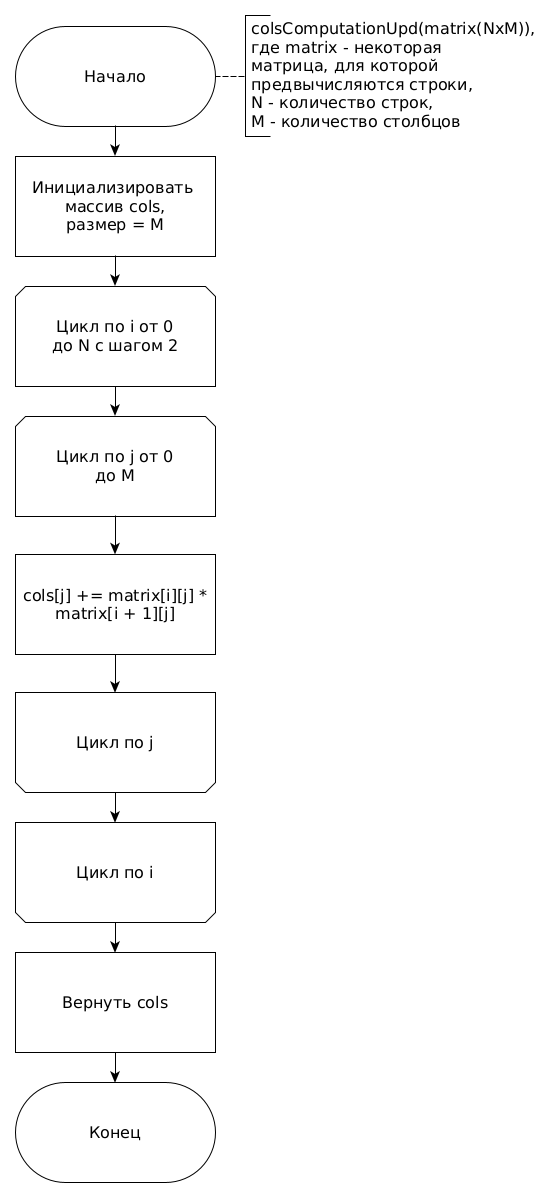
\includegraphics[scale=0.4]{inc/img/colsCompUpd.png}
\captionsetup{justification=centering}
	\caption{Схема предрасчёта столбцов для алгоритма Копперсмита-Винограда.}
	\label{img:colsPreComp}	
\end{center}
\end{figure}
\newpage

\section{Схема алгоритма работы функции, запускающая в требуемом количестве потоков функцию-аргумент}
На рисунке \ref{img:paralFuck} предоставлена схема алгоритма работы функции, запускающей в требуемом количестве потоков функцию-аргумент.

\begin{figure}
\begin{center}
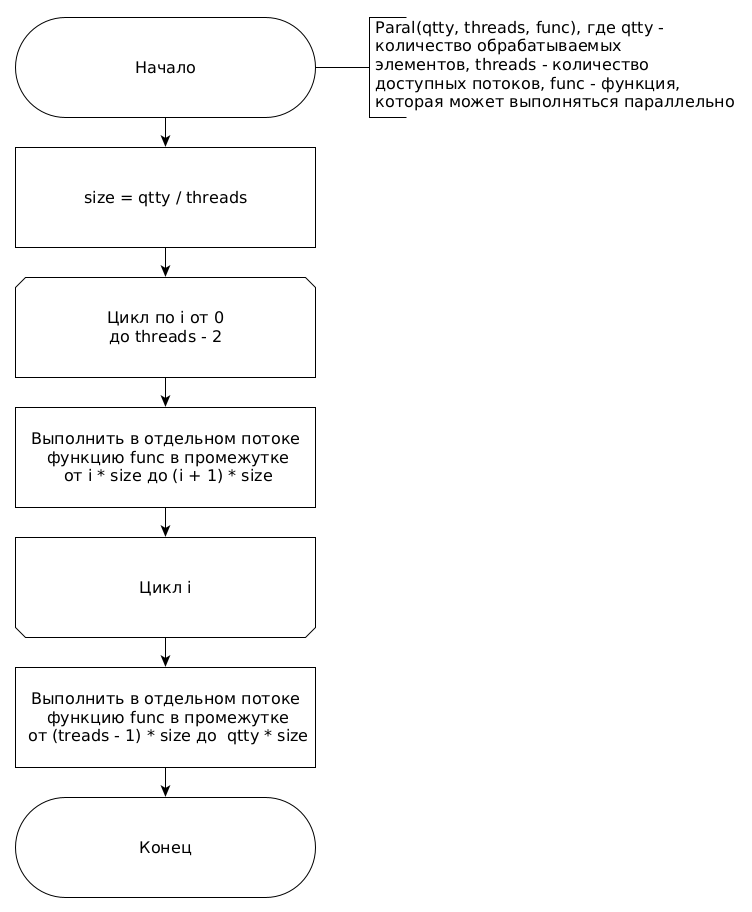
\includegraphics[scale=0.3]{inc/img/paralFunc.png}
\captionsetup{justification=centering}
	\caption{Схема алгоритма работы функции, запускающей в требуемом количестве потоков функцию-аргумент.}
	\label{img:paralFuck}	
\end{center}
\end{figure}

\section{Параллельная реализация алгоритма Копперсмита-Винограда}
Для распараллеливания алгоритма требуется определить, какие из частей алгоритма могут быть выполнены вне зависимости друг от друга.

Часть блок-схемы, отвечающая за предрасчёт строк и столбцов (рисунок \ref{img:paralPart1}), однозначно может быть распараллелен. Но до завершения двух этих подпрограмм к выполнению следующих этапов приступать нельзя, так как вычисленные массивы будут использоваться далее. В данной части будет использоваться полное выделенное количество потоков последовательно - первоначально для вычисления строк, а далее - для вычисления столбцов.
\begin{figure}
\begin{center}
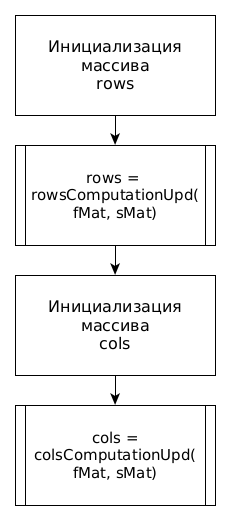
\includegraphics[scale=0.4]{inc/img/paralPart1.png}
\captionsetup{justification=centering}
	\caption{Часть блок-схемы, в которой происходит вызов подпрограмм предрасчёта строк и столбцов.}
	\label{img:paralPart1}	
\end{center}
\end{figure}
\newpage

Непосредственное вычисление значения каждого элемента матрицы, показанное на рисунке \ref{img:paralPart2}, может быть также поэлементно распараллелено. Однако тут важно заметить, что часть данного этапа, показанная на рисунке \ref{img:paralPart21}, и часть, показанная на рисунке \ref{img:paralPart22}, могут быть выполнены как раздельно, так и совместно при обработке каждого из элементов. Важно заметить, что, при раздельном выполнении, потребуется создавать новые потоки, что является достаточно затратным по времени действием.
\begin{figure}
\begin{center}
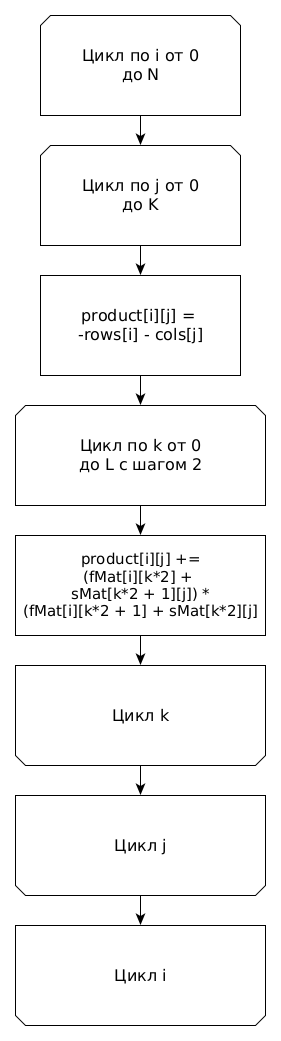
\includegraphics[scale=0.4]{inc/img/paralPart2.png}
\captionsetup{justification=centering}
	\caption{Часть блок-схемы, в которой происходит расчёт значения каждого элемента матрицы.}
	\label{img:paralPart2}	
\end{center}
\end{figure}

\begin{figure}
\begin{center}
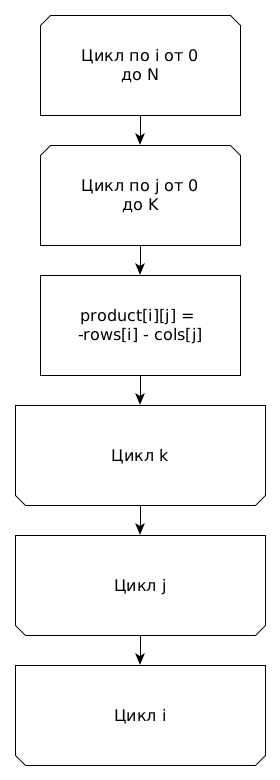
\includegraphics[scale=0.4]{inc/img/paralPart21.png}
\captionsetup{justification=centering}
	\caption{Первая часть рассматриваемого этапа.}
	\label{img:paralPart21}	
\end{center}
\end{figure}

\begin{figure}
\begin{center}
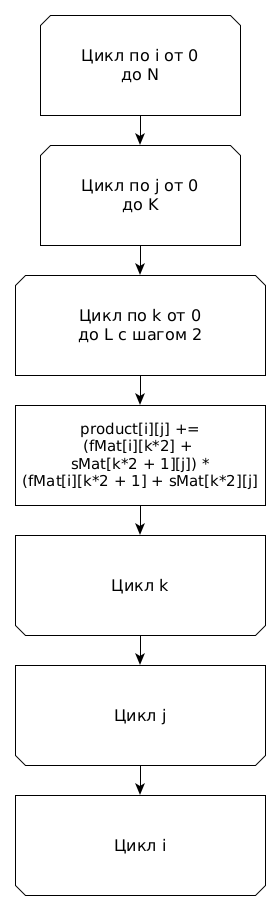
\includegraphics[scale=0.4]{inc/img/paralPart22.png}
\captionsetup{justification=centering}
	\caption{Вторая часть рассматриваемого этапа.}
	\label{img:paralPart22}	
\end{center}
\end{figure}
\newpage

Довычисление значений в случае нечётной размерности итоговой матрицы, показанное на рисунке \ref{img:paralPart3} в каждой итерации цикла требует обращения к матрице, что при распараллеливании приведёт к большому числу блокирований разделяемой памяти и будет неэффективно. Поэтому данный этап останется без изменений.

\begin{figure}
\begin{center}
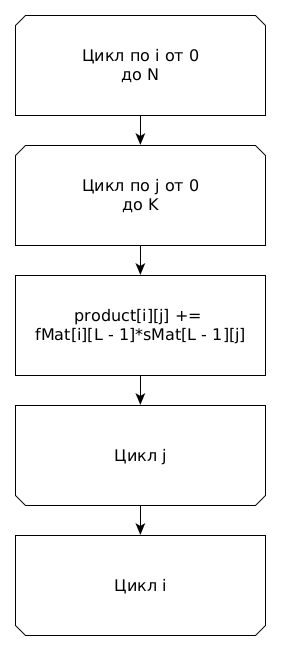
\includegraphics[scale=0.4]{inc/img/paralPart3.png}
\captionsetup{justification=centering}
	\caption{Довычисление значений итоговой матрицы при нечётной размерности оной.}
	\label{img:paralPart3}	
\end{center}
\end{figure}
\newpage

\section{Схема параллельной реализации алгоритма Копперсмита-Винограда с разделением этапа вычисления элементов матрицы}
На рисунке \ref{img:scheme1} предоставлена схема с одновременным выполнением двух частей этапа вычисления элементов матрицы.

\begin{figure}
\begin{center}
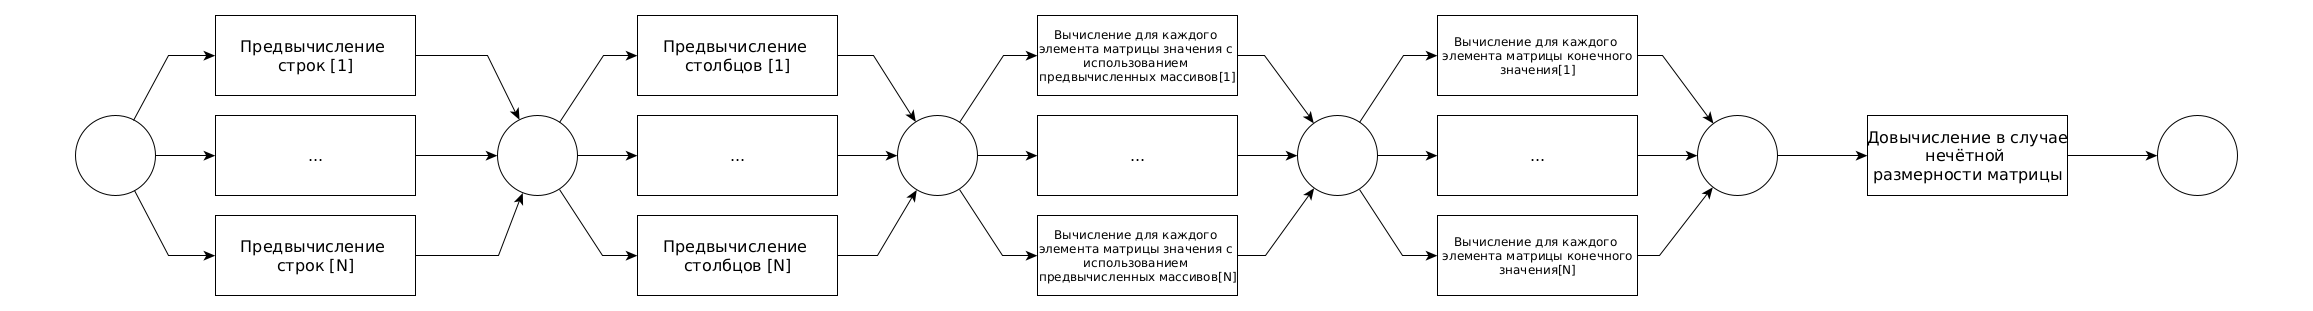
\includegraphics[scale=0.21]{inc/img/paralScheme1.png}
\captionsetup{justification=centering}
	\caption{Схема с одновременным выполнением двух частей этапа вычисления элементов матрицы.}
	\label{img:scheme1}	
\end{center}
\end{figure}
\newpage

\section{Схема параллельной реализации алгоритма Копперсмита-Винограда без разделения этапа вычисления элементов матрицы}
На рисунке \ref{img:scheme2} предоставлена схема с последовательным выполнением двух частей этапа вычисления элементов матрицы.

\begin{figure}
\begin{center}
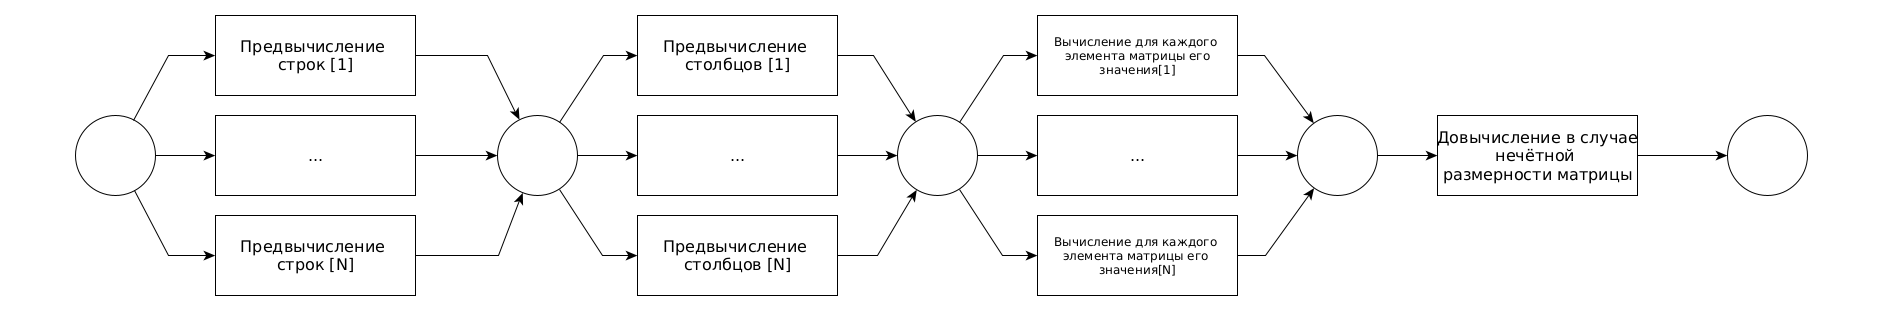
\includegraphics[scale=0.27]{inc/img/paralScheme2.png}
\captionsetup{justification=centering}
	\caption{Схема с последовательным выполнением двух частей этапа вычисления элементов матрицы.}
	\label{img:scheme2}	
\end{center}
\end{figure}
\newpage

\section*{Вывод}
На основе теоретических данных, полученных из аналитического раздела, была построена схема алгоритма Копперсмита-Винограда. Были предложены 2 схемы параллельной реализации рассматриваемого алгоритма.

\chapter{Технологическая часть}
\section{Требования к программному обеспечению}
\begin{itemize}
\item входные данные - две матрицы размерностью $MxN$ и $KxL$;
\item выходные данные - результат умножения двух переданных матриц.
\end{itemize}

\section{Средства реализации программного обеспечения}
При написании программного продукта был использован язык программирования Nim \cite{Nim}.

Данный выбор обусловлен следующими факторами:
\begin{itemize}
\item Компилируемость языка в C, C++, Objective C и JavaScript;
\item Синтаксис языка близок к синтаксису ЯП Python.
\end{itemize}

Для тестирования производительности реализаций алгоритмов использовалась библиотека times.

При написании программного продукта использовалась среда разработки IntelliJ IDEA.

Данный выбор обусловлен тем, что данная среда разработки имеет плагин поддержки языка программирования Nim.

\section{Листинг кода}
В листингах \ref{list:winogradClassic} - \ref{list:paral2} предоставлены реализации рассматриваемых алгоритмов.
\begin{lstlisting}[caption=Алгоритм Копперсмита-Винограда в последовательной реализации,
label={list:winogradClassic}]
proc rowsComp(matrix : seq[seq[int]]) : seq[int]=
    var computedRows = newSeq[int](matrix.len)

    for i in 0..matrix.len - 1:
        var j = 0
        while j < matrix[0].len - 1:
            computedRows[i] += matrix[i][j] * matrix[i][j + 1]
            j += 2

    return computedRows

proc colsComp(matrix : seq[seq[int]]) : seq[int]=
    var computedCols = newSeq[int](matrix[0].len)

    var i = 0
    while i < matrix.len - 1:
        for j in 0..matrix[0].len - 1:
            computedCols[j] += matrix[i][j] * matrix[i + 1][j]
        i += 2

    return computedCols

proc winogradMult(fMat : seq[seq[int]], sMat : seq[seq[int]]) : seq[seq[int]]=
    if (fMat[0].len != sMat.len):
        return

    var computedRows = rowsComp(fMat)
    var computedCols = colsComp(sMat)

    var product = newSeqWith(fMat.len, newSeq[int](sMat[0].len))
    for i in 0..product.len - 1:
        for j in 0..product[0].len - 1:
            product[i][j] += -computedRows[i] - computedCols[j]

            var k = 0
            while k < sMat.len - 1:
                product[i][j] += (fMat[i][k] + sMat[k + 1][j]) * (fMat[i][k + 1] + sMat[k][j])
                k += 2

    if sMat.len %% 2 != 0:
        var curK = sMat.len - 1
        for i in 0..product.len - 1:
            for j in 0..product[0].len - 1:
                product[i][j] += fMat[i][curK] * sMat[curK][j]

    return product
\end{lstlisting}

\begin{lstlisting}[caption=Реализация первой схемы параллельного алгоритма Копперсмита-Винограда,
label={list:paral}]
proc rowsCompThreadFunc(info: tuple[startOfInterval, endOfInterval : int, computedRows : ptr seq[int], matrix : seq[seq[int]]])=
    for i in info.startOfInterval..info.endOfInterval - 1:
        var j = 0
        while j < info.matrix[0].len - 1:
            info.computedRows[i] += info.matrix[i][j] * info.matrix[i][j + 1]
            j += 2

proc rowsCompParallel(matrix : seq[seq[int]]) : seq[int]=
    var compRows = newSeq[int](matrix.len)
    var compRowsPtr = addr compRows
    var thr : array[0..THREADS, Thread[tuple[startOfInterval, endOfInterval: int, computedRows : ptr seq[int], matrix : seq[seq[int]]]]]
    var size = (matrix.len / THREADS).int
    for i in 0..thr.len - 2:
        createThread(thr[i], rowsCompThreadFunc, (i * size, (i + 1) * size, compRowsPtr, matrix))

    createThread(thr[thr.len - 1], rowsCompThreadFunc, ((thr.len - 1) * size, matrix.len, compRowsPtr, matrix))

    joinThreads(thr)
    return compRows

proc colsCompThreadFunc(info : tuple[startOfInterval, endOfInterval : int, computedCols : ptr seq[int], matrix : seq[seq[int]]])=
    var i = 0
    while i < info.matrix.len - 1:
        for j in info.startOfInterval..info.endOfInterval - 1:
            info.computedCols[j] += info.matrix[i][j] * info.matrix[i + 1][j]
        i += 2


proc colsCompParallel(matrix : seq[seq[int]]) : seq[int]=
    var compCols = newSeq[int](matrix[0].len)
    var compColsPtr = addr compCols
    var thr : array[0..THREADS, Thread[tuple[startOfInterval, endOfInterval: int, computedCols : ptr seq[int], matrix : seq[seq[int]]]]]
    var size = (matrix[0].len / THREADS).int
    for i in 0..thr.len - 2:
        createThread(thr[i], colsCompThreadFunc, (i * size, (i + 1) * size, compColsPtr, matrix))

    createThread(thr[thr.len - 1], colsCompThreadFunc, ((thr.len - 1) * size, matrix[0].len, compColsPtr, matrix))

    joinThreads(thr)
    return compCols


proc prepareThreadProd(info : tuple[startOfInterval, endOfInterval: int, product : ptr seq[seq[int]], computedRows, computedCols : seq[int]]) {.thread.}=
    for i in info.startOfInterval..info.endOfInterval - 1:
        for j in 0..info.product[0].len - 1:
                info.product[i][j] += -info.computedRows[i] - info.computedCols[j]

proc finThreadProd(info : tuple[startOfInterval, endOfInterval: int, product : ptr seq[seq[int]], fMat, sMat : seq[seq[int]]]) {.thread.}=
    for i in info.startOfInterval..info.endOfInterval - 1:
        var k = 0
        for j in 0..info.product[0].len - 1:
            k = 0
            while k < info.sMat.len - 1:
                info.product[i][j] += (info.fMat[i][k] + info.sMat[k + 1][j]) * (info.fMat[i][k + 1] + info.sMat[k][j])
                k += 2


proc multParallelFirst(fMat : seq[seq[int]], sMat : seq[seq[int]], computedRows, computedCols : seq[int]) : seq[seq[int]]=
    var product = newSeqWith(fMat.len, newSeq[int](sMat[0].len))

    var prodPtr = addr product
    var fThr : array[0..THREADS, Thread[tuple[startOfInterval, endOfInterval : int, product : ptr seq[seq[int]], computedRows, computedCols : seq[int]]]]
    var size = (product.len / THREADS).int
    for i in 0..fThr.len - 2:
        createThread(fThr[i], prepareThreadProd, (i * size, (i + 1) * size, prodPtr, computedRows, computedCols))
    createThread(fThr[fThr.len - 1], prepareThreadProd, ((fThr.len - 1) * size, product.len, prodPtr, computedRows, computedCols))
    joinThreads(fThr)

    var sThr : array[0..THREADS, Thread[tuple[startOfInterval, endOfInterval : int, product : ptr seq[seq[int]], fMat, sMat : seq[seq[int]]]]]
    for i in 0..sThr.len - 2:
        createThread(sThr[i], finThreadProd, (i * size, (i + 1) * size, prodPtr, fMat, sMat))
    createThread(sThr[sThr.len - 1], finThreadProd, ((sThr.len - 1) * size, product.len, prodPtr, fMat, sMat))
    joinThreads(sThr)

    if sMat.len %% 2 != 0:
        var curK = sMat.len - 1
        for i in 0..product.len - 1:
            for j in 0..product[0].len - 1:
                product[i][j] += fMat[i][curK] * sMat[curK][j]

    return product


proc winogradMultParallelFirst(fMat : seq[seq[int]], sMat : seq[seq[int]]) : seq[seq[int]]=
    if (fMat[0].len != sMat.len):
        return

    var computedRows = rowsCompParallel(fMat)
    var computedCols = colsCompParallel(sMat)

    var product = multParallelFirst(fMat, sMat, computedRows, computedCols)

    return product
\end{lstlisting}

\begin{lstlisting}[caption=Реализация второй схемы параллельного алгоритма Копперсмита-Винограда,
label={list:paral2}]
proc twinThreadProd(info : tuple[startOfInterval, endOfInterval : int, product : ptr seq[seq[int]], computedRows, computedCols : seq[int], fMat, sMat : seq[seq[int]]]) {.thread.}=
    for i in info.startOfInterval..info.endOfInterval - 1:
        for j in info.startOfInterval..info.endOfInterval - 1:
            info.product[i][j] += -info.computedRows[i] - info.computedCols[j]
            var k = 0
            while k < info.sMat.len - 1:
                info.product[i][j] += (info.fMat[i][k] + info.sMat[k + 1][j]) * (info.fMat[i][k + 1] + info.sMat[k][j])
                k += 2

proc multParallelSecond(fMat : seq[seq[int]], sMat : seq[seq[int]], computedRows, computedCols : seq[int]) : seq[seq[int]]=
    var product = newSeqWith(fMat.len, newSeq[int](sMat[0].len))

    var prodPtr = addr product
    var thr : array[0..THREADS, Thread[tuple[startOfInterval, endOfInterval : int, product : ptr seq[seq[int]], computedRows, computedCols : seq[int], fMat, sMat : seq[seq[int]]]]]
    var size = (product.len / THREADS).int
    for i in 0..thr.len - 2:
        createThread(thr[i], twinThreadProd, (i * size, (i + 1) * size, prodPtr, computedRows, computedCols, fMat, sMat))
    createThread(thr[thr.len - 1], twinThreadProd, ((thr.len - 1) * size, product.len, prodPtr, computedRows, computedCols, fMat, sMat))
    joinThreads(thr)

    if sMat.len %% 2 != 0:
        var curK = sMat.len - 1
        for i in 0..product.len - 1:
            for j in 0..product[0].len - 1:
                product[i][j] += fMat[i][curK] * sMat[curK][j]

    return product

proc winogradMultParallelSecond(fMat : seq[seq[int]], sMat : seq[seq[int]]) : seq[seq[int]]=
    if (fMat[0].len != sMat.len):
        return

    var computedRows = rowsCompParallel(fMat)
    var computedCols = colsCompParallel(sMat)

    var product = multParallelSecond(fMat, sMat, computedRows, computedCols)

    return product
\end{lstlisting}

\section{Тестирование программного продукта}
В таблице~\ref{tabular:test_rec} приведены тесты для функций, реализующих алгоритм Копперсмита-Винограда. Тесты пройдены успешно.

\begin{table}[h!]
	\begin{center}
	
	\caption{\label{tabular:test_rec} Тестирование функций}
		\begin{tabular}{c@{\hspace{7mm}}c@{\hspace{7mm}}c@{\hspace{7mm}}c@{\hspace{7mm}}c@{\hspace{7mm}}c@{\hspace{7mm}}}
			\hline
			Матрица 1 & Матрица 2 &Ожидаемый результат \\ \hline
			\vspace{4mm}
			$\begin{pmatrix}
			1 & 2 & 3\\
			1 & 2 & 3\\
			1 & 1 & 1
			\end{pmatrix}$ &
			$\begin{pmatrix}
			1 & 3 & 3\\
			1 & 3 & 3\\
			1 & 2 & 2
			\end{pmatrix}$ &
			$\begin{pmatrix}
			6 & 15 & 15\\
			6 & 15 & 15\\
			3 & 8 & 8
			\end{pmatrix}$ \\
			\vspace{2mm}
			\vspace{2mm}
			$\begin{pmatrix}
            1 & 2 & 4\\
            1 & 2 & 4
			\end{pmatrix}$ &
			$\begin{pmatrix}
			4\\
			5\\
            6
			\end{pmatrix}$ &
			$\begin{pmatrix}
			32\\
			32
			\end{pmatrix}$ \\
			\vspace{2mm}
			\vspace{2mm}
			$\begin{pmatrix}
			5
			\end{pmatrix}$ &
			$\begin{pmatrix}
			666
			\end{pmatrix}$ &
			$\begin{pmatrix}
			3330
			\end{pmatrix}$ \\
			\vspace{2mm}
			\vspace{2mm}
			$\begin{pmatrix}
			-1 & -2 & 3\\
			1 & 2 & 3\\
			-1 & -2 & 3
			\end{pmatrix}$ &
			$\begin{pmatrix}
			1 & 1 & 1\\
			2 & 2 & 2\\
			3 & 3 & 3
			\end{pmatrix}$ &
			$\begin{pmatrix}
			4 & 4 & 4\\
			14 & 14 & 14\\
			4 & 4 & 4
			\end{pmatrix}$\\
			\vspace{2mm}
			\vspace{2mm}
			$\begin{pmatrix}
			666 & 666
			\end{pmatrix}$ &
			$\begin{pmatrix}
			777 & 777
			\end{pmatrix}$ &
			Ошибка\\
		\end{tabular}
	\end{center}
\end{table}
\section*{Вывод}
Спроектированные алгоритмы были реализованы и протестированы.

\chapter{Исследовательская часть}

\section{Пример работы программного обеспечения}
Ниже на рисунках \ref{img:example1}-\ref{img:example2} предоставлены примеры работы каждого из алгоритмов на введённых пользователем данных.

\begin{figure}
\begin{center}
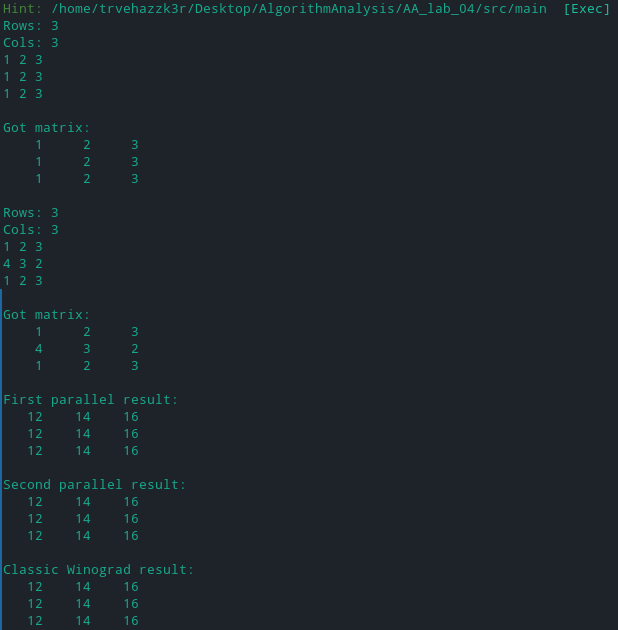
\includegraphics[]{inc/img/example1.png}
\captionsetup{justification=centering}
	\caption{Пример работы ПО.}
	\label{img:example1}	
\end{center}
\end{figure}

\begin{figure}
\begin{center}
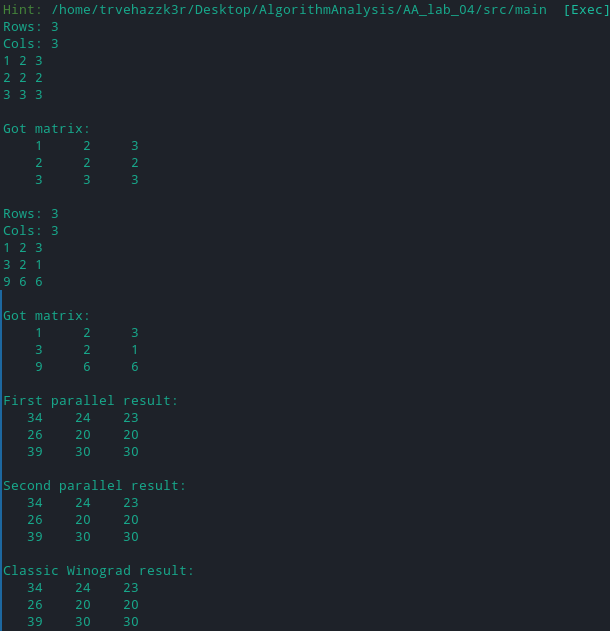
\includegraphics[]{inc/img/example2.png}
\captionsetup{justification=centering}
	\caption{Пример работы ПО.}
	\label{img:example2}	
\end{center}
\end{figure}

\newpage

\section{Технические характеристики}
Технические характеристики ЭВМ, на котором выполнялись исследования:
\begin{itemize}
\item ОС: Manjaro Linux 20.1.1 Mikah
\item Оперативная память: 16 Гб
\item Процессор: Intel Core i7-10510U
\end{itemize}


При проведении замеров времени ноутбук был подключен к сети электропитания.

\section{Время выполнения алгоритмов}
Алгоритмы тестировались на данных, сгенерированных случайным образом.

Результаты замеров времени приведены в таблицах \ref{time1} - \ref{time5}. На рисунках \ref{timeRes1} и \ref{timeRes5} приведены графики зависимостей времени работы алгоритмов от размерности обрабатываемых матриц при 1, 2, 4, 8, 16 потоках. В таблице КВ - последовательный алгоритм Копперсмита-Винограда, Парал1КВ - реализация схемы \ref{img:scheme1} параллельного алгоритма Копперсмита-Винограда, Парал2КВ - реализация схемы \ref{img:scheme2} параллельного алгоритма.

\newpage
\begin{table}[h]
	\begin{center}
		\caption{\label{time1} Замеры времени для различных размеров массивов на 1 потоке.}
		\begin{tabular}{|c |c |c |c|} 
 			\hline
 			&\multicolumn{3}{|c|}{Время работы, нс}\\
 			\hline
			Размеры матрицы & КВ & Парал1КВ & Парал2КВ \\ [0.5ex] 
 			\hline\hline
 			100 & 4692982 & 6144734 & 6125329 \\
 			\hline
 			200 & 49620266 & 56025172 & 58077386 \\
 			\hline
			300 & 178730542 & 199925329 & 206518482 \\
			\hline
			400 & 429056319 & 456832433 & 561695647 \\
			\hline
			500 & 856058247 & 737473554 & 673711435 \\
			\hline
			\end{tabular}
	\end{center}
\end{table}

\begin{table}[h]
	\begin{center}
		\caption{\label{time2} Замеры времени для различных размеров массивов на 2 потоках.}
		\begin{tabular}{|c |c |c |c|} 
 			\hline
 			&\multicolumn{3}{|c|}{Время работы, нс}\\
 			\hline
			Размеры матрицы & КВ & Парал1КВ & Парал2КВ \\ [0.5ex] 
 			\hline\hline
 			100 & 4250527 & 4315274 & 2910312\\
 			\hline
 			200 & 50728798 & 34809356 & 18273241 \\
 			\hline
			300 & 186202130 & 120880876 & 61885504 \\
			\hline
			400 & 436860056 & 248104438 & 137340969 \\
			\hline
			500 & 870833440 & 576761740 & 267199177 \\
			\hline
			\end{tabular}
	\end{center}
\end{table}

\begin{table}[h]
	\begin{center}
		\caption{\label{time3} Замеры времени для различных размеров массивов на 4 потоках.}
		\begin{tabular}{|c |c |c |c|} 
 			\hline
 			&\multicolumn{3}{|c|}{Время работы, нс}\\
 			\hline
			Размеры матрицы & КВ & Парал1КВ & Парал2КВ \\ [0.5ex] 
 			\hline\hline
 			100 & 4485824 & 4239416 & 2969518 \\
 			\hline
 			200 & 51678241 & 28600648 & 10260636 \\
 			\hline
			300 & 176448578 & 80224609 & 31277241 \\
			\hline
			400 & 436787067 & 208705553 & 70302333 \\
			\hline
			500 & 850999256 & 485612161 & 151094601 \\
			\hline
			\end{tabular}
	\end{center}
\end{table}

\begin{table}[h]
	\begin{center}
		\caption{\label{time4} Замеры времени для различных размеров массивов на 8 потоке.}
		\begin{tabular}{|c |c |c |c|} 
 			\hline
 			&\multicolumn{3}{|c|}{Время работы, нс}\\
 			\hline
			Размеры матрицы & КВ & Парал1КВ & Парал2КВ \\ [0.5ex] 
 			\hline\hline
 			100 & 4403638 & 5304634 & 3712704 \\
 			\hline
 			200 & 52234883 & 26568390 & 11046163 \\
 			\hline
			300 & 177331754 & 107137650 & 31637714 \\
			\hline
			400 & 442171563 & 337629280 & 58383234 \\
			\hline
			500 & 877219464 & 883596315 & 117636357 \\
			\hline
			\end{tabular}
	\end{center}
\end{table}

\begin{table}[h]
	\begin{center}
		\caption{\label{time5} Замеры времени для различных размеров массивов на 16 потоках.}
		\begin{tabular}{|c |c |c |c|} 
 			\hline
 			&\multicolumn{3}{|c|}{Время работы, нс}\\
 			\hline
			Размеры матрицы & КВ & Парал1КВ & Парал2КВ \\ [0.5ex] 
 			\hline\hline
 			100 & 4463337 & 7381390 & 4981564 \\
 			\hline
 			200 & 50528949 & 32361454 &  17479130 \\
 			\hline
			300 & 175677695 & 110593792 & 44960321 \\
			\hline
			400 & 433177913 & 342768739 & 68839512 \\
			\hline
			500 & 831773652 & 887656714 & 100236284 \\
			\hline
			\end{tabular}
	\end{center}
\end{table}
\newpage

\begin{figure}[h]
\begin{center}
	\begin{tikzpicture}

\begin{axis}[
  		  	axis lines = left,
  		  	xlabel = размерность,
  		  	ylabel = {время, нс},
			legend pos=north west,
			ymajorgrids=true
		] 
		\addplot[color=orange] table[x index=0, y index=1] {KB11.dat};
		\addplot[color=blue, mark=square] table[x index=0, y index=1] {KB21.dat};
		\addplot[color=green, mark=square] table[x index=0, y index=1] {KB31.dat};

		\addlegendentry{КВ}
		\addlegendentry{Paral1КВ}
		\addlegendentry{Paral2КВ}
		\end{axis}
	\end{tikzpicture}
	\captionsetup{justification=centering}
	\caption{Зависимость времени работы от размерности матриц (при 1 потоке).}
	\label{timeRes1}
	\end{center}
\end{figure}

\begin{figure}[h]
\begin{center}
	\begin{tikzpicture}
\begin{axis}[
  		  	axis lines = left,
  		  	xlabel = размерность,
  		  	ylabel = {время, нс},
			legend pos=north west,
			ymajorgrids=true
		] 
		\addplot[color=orange] table[x index=0, y index=1] {KB12.dat};
		\addplot[color=blue, mark=square] table[x index=0, y index=1] {KB22.dat};
		\addplot[color=green, mark=square] table[x index=0, y index=1] {KB32.dat};

		\addlegendentry{КВ}
		\addlegendentry{Парал1КВ}
		\addlegendentry{Парал2КВ}
		\end{axis}
	\end{tikzpicture}
	\captionsetup{justification=centering}
	\caption{Зависимость времени работы от размерности матриц (при 2 потоках)}
	\label{timeRes2}
	\end{center}
\end{figure}

\begin{figure}[h]
\begin{center}
	\begin{tikzpicture}
\begin{axis}[
  		  	axis lines = left,
  		  	xlabel = размерность,
  		  	ylabel = {время, нс},
			legend pos=north west,
			ymajorgrids=true
		] 
		\addplot[color=orange] table[x index=0, y index=1] {KB14.dat};
		\addplot[color=blue, mark=square] table[x index=0, y index=1] {KB24.dat};
		\addplot[color=green, mark=square] table[x index=0, y index=1] {KB34.dat};

		\addlegendentry{КВ}
		\addlegendentry{Парал1КВ}
		\addlegendentry{Парал2КВ}
		\end{axis}
	\end{tikzpicture}
	\captionsetup{justification=centering}
	\caption{Зависимость времени работы от размерности матриц (при 4 потоках)}
	\label{timeRes3}
	\end{center}
\end{figure}

\begin{figure}[h]
\begin{center}
	\begin{tikzpicture}
\begin{axis}[
  		  	axis lines = left,
  		  	xlabel = размерность,
  		  	ylabel = {время, нс},
			legend pos=north west,
			ymajorgrids=true
		] 
		\addplot[color=orange] table[x index=0, y index=1] {KB18.dat};
		\addplot[color=blue, mark=square] table[x index=0, y index=1] {KB28.dat};
		\addplot[color=green, mark=square] table[x index=0, y index=1] {KB38.dat};

		\addlegendentry{КВ}
		\addlegendentry{Парал1КВ}
		\addlegendentry{Парал2КВ}
		\end{axis}
	\end{tikzpicture}
	\captionsetup{justification=centering}
	\caption{Зависимость времени работы от размерности матриц (при 8 потоках)}
	\label{timeRes4}
	\end{center}
\end{figure}

\begin{figure}[h]
\begin{center}
	\begin{tikzpicture}
\begin{axis}[
  		  	axis lines = left,
  		  	xlabel = размерность,
  		  	ylabel = {время, нс},
			legend pos=north west,
			ymajorgrids=true
		] 
		\addplot[color=orange] table[x index=0, y index=1] {KB116.dat};
		\addplot[color=blue, mark=square] table[x index=0, y index=1] {KB216.dat};
		\addplot[color=green, mark=square] table[x index=0, y index=1] {KB316.dat};

		\addlegendentry{КВ}
		\addlegendentry{Парал1КВ}
		\addlegendentry{Парал2КВ}
		\end{axis}
	\end{tikzpicture}
	\captionsetup{justification=centering}
	\caption{Зависимость времени работы от размерности матриц (при 16 потоках)}
	\label{timeRes5}
	\end{center}
\end{figure}

\newpage

\section*{Вывод}
При сравнении результатов замеров по времени видно, что рассматривать скорость работы распараллеленных алгоритмов на одном потоке смысла нет, так как они работают медленнее на $\approx 16\%$. Связанно это с тем, что на создание потоков тратится время.

На 2-х потоках обе схемы себя показывают уже лучше. Схема распараллеливания с разделением показывает себя хуже, чем вторая схема, на $\approx 181\%$ (на размерности 300). При этом последовательная реализация будет работать медленнее схемы без разделения на $\approx 326\%$.

На 4-х потоках схемы вновь показывают себя лучше. При этом они работают быстрее, чем на 2-х потоках. Схема распараллеливания с разделением показывает себя хуже, чем вторая схема, на $\approx 297\%$.

На 8-и потоках первая схема показывает себя уже хуже, чем на 4-х потоках. Таким образом 4 потока - это оптимальный вариант решения задачи для первой схемы. Такое увеличение времени выполнения может связано со временем, затрачиваемым на создание потоков. Схема распараллеливания с разделением показывает себя хуже, чем вторая схема на $\approx 578\%$.

На 16-ти потоках схемы работают с ещё меньшей эффективностью. Схема распараллеливания с разделением показывает себя хуже второй реализации на $\approx 500\%$.  Таким образом, вторая реализация параллельной схемы уже начинает несколько уменьшать своё преимущество, но при этом она всё ещё имеет свой потенциал.

Таким образом, параллельная реализация действительно работает быстрее последовательной. Но важно отметить факт того, что требуется ответственно относиться к выделяемым ресурсам.

\chapter*{Заключение}
\addcontentsline{toc}{chapter}{Заключение}
В ходе выполнения лабораторной работы была выполнена цель и следующие задачи:
\begin{enumerate}
\item были изучены последовательный и два параллельных реализаций алгоритмов Копперсмита-Винограда;
\item были реализованы последовательный и два параллельных алгоритма Копперсмита-Винограда;
\item был проведён сравнительный анализ алгоритмов на основе экспериментальных данных;
\item был подготовлен отчёт по лабораторной работе;
\item были получены практические навыки реализации алгоритмов на ЯП Nim.
\end{enumerate}

Исследования показали, что первая схема параллельной реализации показывает себя в среднем на $\approx 445\%$ хуже реализации с неразделённым вычислением элементов итоговой матрицы. Связано это с повторным выделением потоков для решения дополнительной задачи. Также стало известно, что в случае рассмотрения разницы между последовательной реализацией и параллельной с неразделённым вычислением элементов итоговой матрицы, первая покажет себя хуже в среднем на $\approx 322\%$

\addcontentsline{toc}{chapter}{Литература}
\bibliographystyle{utf8gost705u}  % стилевой файл для оформления по ГОСТу
\bibliography{biblio.bib}          % имя библиографической базы (bib-файла)


\end{document} 
